Para melhor compreensão do texto, é importante estabelecer as definições de alguns conceitos que serão adotados neste projeto de pesquisa. 

\begin{comment}{
{\color{red}[MODELO]
\index{elementos textuais} O Referencial Teórico é um seção dos elementos textuais. A norma ABNT NBR 15287:2011, p. 5, apresenta a
seguinte orientação quanto aos elementos textuais:

\begin{citacao}
O texto deve ser constituído de uma parte introdutória, na qual devem ser
expostos o tema do projeto, o problema a ser abordado, a(s) hipótese(s),
quando couber(em), bem como o(s) objetivo(s) a ser(em) atingido(s) e a(s)
justificativa(s). É necessário que sejam indicados o referencial teórico que
o embasa, a metodologia a ser utilizada, assim como os recursos e o cronograma
necessários à sua consecução.\citeonline{abntex2classe}
\end{citacao}, ,

Deve-se apresentar a fundamentação teórica que orientará o estudo. Recomenda-se situar a grande área, subárea e objeto de estudo. Se for necessário pode ser feito um resgate histórico para demonstrar a evolução da área. Faz-se necessário relatar o momento vivido pela área (Marco Teórico - Estado da Arte) geralmente intitulado de Trabalhos Relacionados.

O Referencial Teórico é considerado como um elemento de controle de toda a pesquisa, desde a problematização inicial. O pesquisador irá interpretar seu objeto de estudo de acordo com a concepção teórica de uma ou toda a obra de um autor ou de um objeto ou produto ou de um conjunto de autores (esta condução varia de acordo com cada área de conhecimento). Todas as etapas do projeto são definidas conforme esta escolha. Apresenta-se de modo aprofundado, respondendo quais os princípios, categorias, conceitos ou teorias fundamentam a pesquisa. Deve estar de acordo com o tema formulado e o raciocínio desenvolvido nas fases anteriores. 

}}\end{comment}

\section{Educação de Computação}
\label{sec:EC}

Educação de computação é o resultado da fusão de, a princípio --- Outras também estão envolvidas, como: Psicologia, engenharias, tecnologia, entre outras ---, duas disciplinas: Educação e Computação. 

Educação é um processo que visa o desenvolvimento físico, intelectual e moral do ser humano, através da aplicação de métodos próprios, com intuito de assegurar-lhe a integração social e formal da cidadania \cite{weiszflog1999michaelis}. Ciência da Computação é o estudo sistemático de algoritmo e estrutura de dados, i.e., o estudo do seu formalismo, desenvolvimento e aplicações \cite{gibbs1986model}. O objetivo principal da pesquisa em Educação de Computação é o aperfeiçoamento do processo de ensino e aprendizagem da Computação como ciência \cite{holmboe2001research}.

\citeonline{fincher2005mapping} identificam dez grandes áreas de interesse para pesquisadores em Educação de Computação. As dez áreas são: a compreensão do aluno, sistemas de animação/visualização/simulação, métodos de ensino, avaliação, tecnologia educacional, a transferência de prática profissional em sala de aula, a incorporação de um novo desenvolvimento e novas tecnologias na sala de aula, transferindo para o ensino à distância (“EaD” ou “\textit{e-learning}”), recrutamento e retenção de alunos, a construção da disciplina à distância (“EaD” ou “\textit{e-learning}”) e, finalmente, a construção da disciplina em si. 

%Artigos ============================
%{\color{red}LER}\cite{da2014metodos}

\section{Avaliação}
\label{sec:AVA}
A avaliação é uma área ampla, que pode ser dividida em termos de tipos de avaliação, validade da avaliação e classificação automatizada \cite{fincher2005mapping}. Segundo \citeonline{libaneo1994didatica}, avaliação pode ser definida como um componente do processo de ensino que visa, através da verificação e qualificação dos resultados obtidos, determinar a correspondência  deste com os objetivos propostos e, daí, orientar a tomada de decisões em relação às atividades didáticas subsequentes.

Outra definição foi dada por \citeonline{domingos1981forma}, onde a avaliação pode ser entendida como um processo sistemático de determinar a extensão em que os objetivos educacionais foram alcançados pelos alunos. O que se avalia são as metas de aprendizagem definidas e para as quais se caminhou durante todo um processo de aprendizagem.

A avaliação da aprendizagem possibilita a tomada de decisão e a melhoria da qualidade de ensino, informando as ações em desenvolvimento e a necessidade de regulações constantes \cite{kraemer2005avaliaccao}.

Para \citeonline{datrino2015avaliaccao}, a avaliação vista como uma etapa da aprendizagem passa a ser utilizada como um processo, i.e., na formação e construção do conhecimento levando a uma reflexão sobre as ações, gestos e pensamentos. Os processos formativos precisam ser avaliados em sua forma, efeito, método e evolução dos educandos.

Os métodos avaliativos são de suma importância no processo de ensino-aprendizagem. Diversos autores demonstram os benefícios resultantes de uma boa avaliação durante as aprendizagens e conhecimentos adquiridos pelos discentes. Porém, é preciso que sejam escolhidos e aplicados no cotidiano do aluno de forma a conduzi-lo à aprendizagem, obtendo assim resultados satisfatórios a partir de sua avaliação e evitando análises errôneas e estresse por parte dos educadores e educandos \cite{da2014alunos}.

Segundo \citeonline{libaneo1994didatica}, o entendimento correto da avaliação consiste em considerar a relação mútua entre os aspectos quantitativos e qualitativos. A avaliação não pode ser vista apenas como ``medida'', mas também não pode ser baseada na subjetividade de professores e alunos. \citeonline{bloom1983manual} classificaram a avaliação em três tipos, sendo eles: avaliação diagnóstica; avaliação formativa e avaliação somativa. estes serão descritos a seguir.

\subsection{Avaliação diagnóstica}
\label{sec:AvaDiag}
Conhecer o aluno, seus gostos, seus hábitos e suas preferências, é o princípio base da avaliação diagnóstica. Dessa forma, assegura-se que o aluno esteja na turma correta e que o curso encontre-se no nível adequado a ele. Nesta avaliação busca-se conhecer ideias e conhecimentos prévios do aluno \cite{masetto1994didatica}.

Para \citeonline{bloom1983manual}, avaliação diagnóstica visa verificar a existência, ou ausência, de habilidades e conhecimentos preestabelecidos. Esta é uma ação que inicia o processo avaliativo e verifica se os alunos dominam os pré‐requisitos necessários para novas aprendizagens.

Segundo \citeonline{haydtavaliaccao}, a partir de uma avaliação diagnóstica o docente constata se os seus alunos estão ou não preparados e se possuem domínio de pré–requisitos para adquirir novos conhecimentos. Portanto, a avaliação diagnóstica permite que o professor conheça seu aluno por um mecanismo de triagem e calibração.

\subsection{Avaliação somativa}
\label{sec:AvaSom}
Avaliação somativa é uma decisão que leva em conta a soma de um ou mais resultados e pode ser baseada numa só prova final \cite{e2004aprender}. Já de acordo com \citeonline{haydtavaliaccao}, esse tipo de avaliação tem por princípio classificar os resultados de aprendizagem alcançados pelos alunos de acordo com os níveis de aproveitamento estabelecidos, adotando assim uma função classificatória.

Para \citeonline{kraemer2005avaliaccao}, a avaliação somativa pretende ajuizar o progresso realizado pelo aluno, no final de uma unidade de aprendizagem, no sentido de aferir resultados já recolhidos por avaliações do tipo formativo e obter indicadores que permitam aperfeiçoar o processo de ensino.

\subsection{Avaliação formativa}
\label{sec:AvaFor}
A ideia de avaliação formativa é sistematizar o funcionamento, levando o professor a observar mais metodicamente os alunos, a compreender melhor seus funcionamentos, de modo a ajustar de maneira mais sistemática e individualizada suas intervenções pedagógicas e as situações didáticas que propõe, tudo isso na expectativa de otimizar a aprendizagem. 

A avaliação formativa está portanto centrada essencialmente, direta e imediatamente, sobre a gestão das aprendizagens dos alunos (pelo professor e pelos interessados). Essa concepção se situa abertamente na perspectiva de uma regulação intencional, cuja intenção seria determinar ao mesmo tempo o caminho já percorrido por cada um e aquele que resta a percorrer com vistas a intervir para otimizar os processos de aprendizagem em curso \cite{perrenoud1999avaliaccao}.

A avaliação formativa responde a uma concepção do ensino que considera que aprender é um longo processo, por meio do qual o aluno vai reestruturando seu conhecimento a partir das atividades que executa. Esse tipo de avaliação tem como finalidade fundamental a função ajustadora do processo de ensino-aprendizagem para possibilitar que os meios de formação respondam as características dos alunos. Pretende-se detectar os pontos fracos da aprendizagem, mais do que determinar quais os resultados obtidos com essa aprendizagem \cite{jorba2003funccao}.

\section{Inteligência Artificial}
\label{sec:IA}
A IA (Inteligência Artificial) é uma das ciências mais recentes. O trabalho começou logo após Segunda Guerra Mundial, tendo este nome cunhado em 1956 \cite{russell2004inteligencia}. Segundo \citeonline{bellman1978introduction}, a IA é a automatização de atividades que podem ser associadas ao pensamento humano, atividades como a tomada de decisões, a resolução de problemas, o aprendizado, entre outros.

Várias disciplinas contribuíram com ideias, pontos de vista e técnicas para a IA. Dentre elas estão: Filosofia, Matemática, Economia, Neurociência, Psicologia, Engenharia de Computadores, Teoria de Controle e Cibernética, Linguística, entre outras \cite{russell2004inteligencia}.

A IA abrange uma enorme variedade de subcampos, desde áreas de uso geral, como aprendizado e percepção, até tarefas específicas como diagnóstico de doenças, por exemplo. A IA sistematiza e automatiza tarefas intelectuais e, portanto, é potencialmente relevante para qualquer esfera da atividade intelectual humana \cite{russell2004inteligencia}.

De acordo com \citeonline{sage1990concise}, o objetivo da IA é o desenvolvimento de paradigmas ou algoritmos que requeiram máquinas para realizar tarefas cognitivas, para as quais os humanos são atualmente melhores. Um sistema de IA tem três componentes fundamentais: representação, raciocínio e aprendizagem.

Aprendizado de Máquina é uma área da IA cujo objetivo é o desenvolvimento de técnicas computacionais sobre o aprendizado bem como a construção de sistemas capazes de adquirir conhecimento de forma automática. Um sistema de aprendizado é um programa de computador que toma decisões baseado em experiências acumuladas através da solução bem sucedida de problemas anteriores. Os diversos sistemas de aprendizado de máquina possuem características particulares e comuns que possibilitam sua classificação quanto à linguagem de descrição, modo, paradigma e forma de aprendizado utilizado \cite{monard2003sistemas}.
Umas das técnicas de aprendizado de máquina são as Redes Neurais Artificiais.

%\subsection{Aprendizado de Máquina}

\subsection{Redes Neurais Artificiais}
\label{sec:RNA}

Uma parte do trabalho inicial da IA teve como objetivo criar \textbf{Redes Neurais Artificiais} (RNA) \cite{russell2004inteligencia}. As RNA's podem ser consideradas análogas às conexões sinápticas do cérebro humano, e o conjunto de entrada às células do sistema nervoso, chamadas de neurônios. Nesta seção serão apresentados os conceitos e diferenças envolvidas entre o neurônio biológico e o artficial, definição de Redes Neurais Artificiais, formalizações matemáticas, modelos, ilustrações, e alguns conceitos importantes, como: Processamento de entrada, Aprendizagem, Perceptron, Regra de Delta, Camadas da Rede, Retro-propagação e critérios de avaliação do desempenho da Rede Neural.
{\color{red} MELHORAR TEXTO}
%Estas são funções não-lineares complexas com muitos parâmetros. 

\subsubsection{Neurônio Biológico}
    O cérebro é um computador (Sistema de processamento de informação) altamente complexo, não-linear e paralelo. Ele tem a capacidade de organizar seus constituintes estruturais, chamados de neurônios, de forma a realizar certos processamentos muito mais rápido que o computador mais veloz existente.
    
    O sistema nervoso humano pode ser visto como um sistema de três estágios. O centro do sistema é o cérebro, que recebe continuamente informação, realiza a percepção desta e toma decisões apropriadas. Os receptores convertem estímulos do corpo humano ou do ambiente externo e converte em impulsos elétricos que transmitem informação para a rede neural (cérebro). Os atuadores convertem impulsos elétricos gerados pela rede neural em respostas discerníveis.
    
    Os neurônios são mais lentos que as portas lógicas de silício. Mesmo assim, o cérebro humano espantosamente mais eficiente, devido a quantidade de células nervosas, com conexões maciças entre si. Estima-se que haja aproximadamente 10 bilhões de neurônios no córtex humano e 60 trilhões de sinapses ou conexões \cite{shepherd1990synaptic}. As sinapses são unidades estruturais e funcionais elementares que medeiam as interações entre os neurônios. As figuras \ref{fig:Neuro} e \ref{fig:Neuronio} apresentam ilustrações meramente ilustrativas das estruturas neurais biológicas dos seres humanos.
    
    %{\color{red} Colocar figura de cérebro humano}

    \begin{figure}
    \centering
    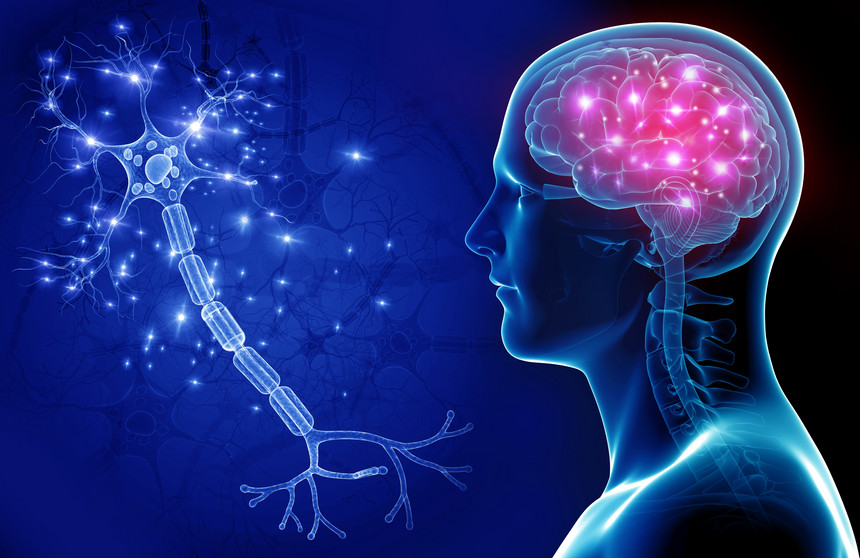
\includegraphics[width=0.9\textwidth]{modelo-monografia-rej-2018/img/mw-860.jpg}
    \caption{Cérebro e neurônio}
    \label{fig:Neuro}
    \end{figure}
    
    \begin{figure}
    \centering
    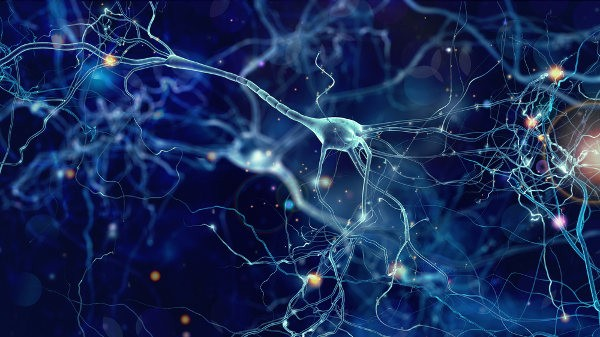
\includegraphics[width=0.9\textwidth]{modelo-monografia-rej-2018/img/neuronio.jpg}
    \caption{Neurônio}
    \label{fig:Neuronio}
    \end{figure}

\subsubsection{Neurônios Artificiais e a Rede Neural Artificial}

 \begin{citacao}
     Uma rede neural é um processador maciçamente paralelamente distribuído constituído de unidades de processamento simples, que têm a propensão natural para armazenar conhecimento experimental e torná-lo disponível para o uso. Ela se assemelha ao cérebro em dois aspectos: Conhecimento adquirido pela rede, através de um processo de aprendizagem, e forças de conexão entre neurônios, conhecidos como pesos sinápticos, usados para armazenar o conhecimento adquirido. \citeonline{haykin2001redes}
 \end{citacao}
 
\citeonline{haykin2001redes} descreveu ainda que a arquitetura de uma rede neural restringe o tipo de problema no qual a rede poderá ser utilizada, e é definida pelo número de camadas (camada única ou múltiplas camadas), pelo número de nós em cada camada, pelo tipo de conexão entre os nós (\textit{feedforward} ou \textit{feedback}) e por sua topologia.

Uma rede neural extrai seu poder computacional através de sua estrutura maciçamente paralelamente distribuída e de sua habilidade de aprender e portanto de generalizar --- refere-se ao fato de a rede neural produzir saídas adequadas para entradas que não estavam presentes durante o treinamento (aprendizagem). O uso de redes neurais fornecem algumas propriedades úteis e capacidades, são elas:

    \begin{enumerate}
        \item {\color{red} TERMINAR}
        \item Não-linearidade:
        \item Mapeamento de Entrada-Saída:
        \item Adaptabilidade:
        \item Resposta à Evidências:
        \item Informação Contextual:
        \item Tolerância a Falhas:
        \item Implementação em VLSI:
        \item Uniformidade de Análise de Projeto:
        \item Analogia Neurobiológica
    \end{enumerate}
    
    Como dito anteriormente, o neurônio é uma unidade de processamento de informação que é fundamental para a operação de uma rede neural. A \autoref{fig:MoudeloNeuroNL} mostra o modelo de um neurônio, que forma a base para o projeto de redes neurais artificiais. Três elementos podem ser identificados na ilustração:
    \begin{itemize}
        \item Um conjunto de sinapses ou conexões, caracterizada por um "peso". O sinal de entrada é multiplicado pelo peso sináptico.
        \item Um somador para somar os sinais de entrada, ponderados pelas respectivas sinapses do neurônio; Um combinador linear.
        \item Uma função de ativação para restringir a amplitude da saída de um neurônio. É também referida como função restritiva já que limita o intervalo permissível de amplitude do sinal de saída a um valor finito.
        \item A figura inclui também um \textit{bias} aplicado externamente, que tem o efeito de aumentar ou diminuir a entrada líquida da função de ativação, dependendo se ele é positivo ou negativo, respectivamente. 
    \end{itemize}
    
    Um neurônio \textit{k} pode ser descrito matematicamente pelo par de equações \ref{eq:uk} e \ref{eq:yk}. Onde ${x_{1}, x_{2}, ..., x_{m}}$ são os sinais de entrada; ${w_{k1}, x_{k2}, ..., x_{km}}$; ${u_{k}}$ é a saída do combinador linear; ${b_{k}}$ é o bias; $\varphi$ é a função de ativação; e ${y_{k}}$ é o sinal de saída do neurônio.
    
    \begin{figure}
    \centering
    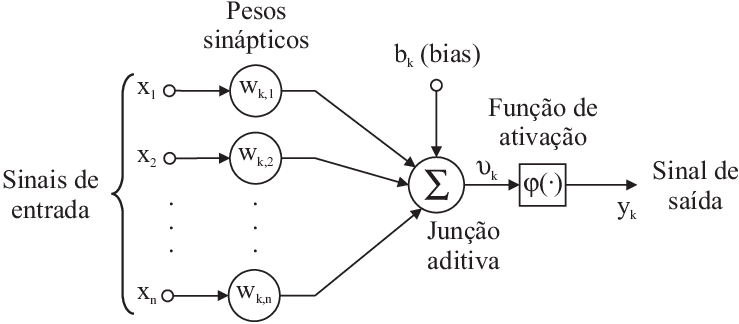
\includegraphics[width=0.9\textwidth]{modelo-monografia-rej-2018/img/Figura-1-Modelo-nao-linear-de-um-neuronio-Haykin-2001.png}
    \caption{Modelo não-linear de um neurônio}
    \label{fig:MoudeloNeuroNL}
    \end{figure}
    
    
    \begin{equation} \label{eq:uk}
        u_{k} = \sum_{j=1}^{m}{w_{kj}x_{j}}     
    \end{equation}
    
    \begin{equation} \label{eq:yk}
        y_{k} = \varphi (u_{k}+b_{k})
    \end{equation}
    
\subsubsection{Arquitetura de Rede}
A maneira pela qual os neurônios de uma rede neural estão estruturados está intimamente ligado com o algoritmo de aprendizagem usado para treinar a rede. Em geral, podemos identificar três classes de arquiteturas de rede diferentes:
    \begin{itemize}
        \item Redes Alimentadas Adiante com Camada Única: A forma mais simples de uma rede em camadas, temos a entrada de nós sobre uma camada de saída de neurônios, mas não vice-versa. Essa rede é chamada de Rede de Camada Única, referindo-se a camada saída de nós computacionais. A ilustração (a) na \autoref{fig:SLPMLP} apresenta uma rede acíclica de camada única.
        \item Redes Alimentadas Diretamente com Múltiplas Camadas: Se distingue pela presença de uma ou mais camadas ocultas. A função dos neurônios ocultos é intervir entre a entrada externa e a saída da rede de uma maneira útil. A ilustração (b) na \autoref{fig:SLPMLP} apresenta uma rede de camadas ocultas, com 10 nós de entrada, 4 camadas ocultas e 2 nós de saída, sendo assim uma rede 10-4-2.
        \item Rede Recorrentes: Se distinguem das duas anteriores por ter pelo menos um laço de realimentação. Uma rede recorrente pode consistir de uma única camada de neurônio com cada neurônio alimentando seu sinal de saida de volta para as entradas.
    \end{itemize}
    
    \begin{figure}
    \centering
    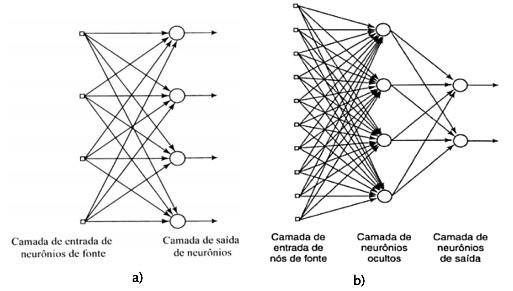
\includegraphics[width=0.9\textwidth]{modelo-monografia-rej-2018/img/Figura-1-a-Rede-de-camada-unica-b-Rede-de-multiplas-camadas.png}
    \caption{Redess Neurais de Camada Única e Múltiplas}
    \label{fig:SLPMLP}
    \end{figure}

\subsubsection{Aprendizagem}
A propriedade que é primordial para uma rede neural é a sua habilidade de aprender e de melhorar o seu desempenho através da aprendizagem. Segundo \citeonline{mendel19708}, a aprendizagem é um processo pelo qual parâmetros livres de uma rede neural são adaptados através de um processo de estimulação pelo ambiente. O tipo de aprendizagem é determinado pela maneira pela qual a modificação ocorre. Um conjunto preestabelecido de regras bem-definidas para a solução de um problema de aprendizagem é chamado de Algoritmo de aprendizagem. Basicamente, os algoritmos diferem entre si pela formulado o ajuste de um peso sináptico de um neurônio. 

Essa definição do processo de aprendizagem implica  a seguinte sequência de eventos:
    \begin{enumerate}
        \item A rede neural é estimulada por um ambiente.
        \item A rede neural sofre modificações nos seus parâmetros livres como resultado desta estimulação.
        \item A rede neural responde de uma maneira nova ao ambiente, devido às modificações ocorridas na sua estrutura interna.
    \end{enumerate}
  
%https://www.maxwell.vrac.puc-rio.br/7587/7587_5.PDF
%http://www.ic.uff.br/~jsilva/monografia_RNA.pdf

\subsubsubsection{Aprendizagem por Correção de Erro}
Neste modelo a correção dos pesos sinápticos é efetuada através da comparação da saída desejada com a saída atual, ambas medidas no mesmo instante de tempo. O erro é então definido com sendo a diferença do valor da saída desejado e a saída atual.

A fim de se estimar o erro da rede define-se uma função custo baseada na função erro. Esta função indica o erro instantâneo da rede e procura-se em adaptar os pesos
sinápticos a fim de minimizar essa função. 

\begin{equation} \label{eq:erro}
    e_{k}(n) = d_{k}(n) - y_{k}(n)    
\end{equation}

A \autoref{eq:erro} descreve a função de erro, onde o sinal de erro $e_{k}(n)$ aciona um mecanismo de controle, com propósito de aplicar uma sequência de ajustes corretivos aos pesos sinápticos do neurônio k. Os ajustes corretivos são projetados para aproximar passo a passo o sinal de saída $y_{k}(n)$ da resposta desejada $d_{k}(n)$. O objetivo é alcançado minimizando-se uma função de custo ou índice de desempenho, E(n), definido em termos do sinal de erro $e_{k}(n)$ como descrito na \autoref{eq:custo}. $E(n)$ é o valor instantâneo da energia do erro. Os ajustes dos pesos sinápticos continuam até o sistema atingir um estado estável.

\begin{equation} \label{eq:custo}
    E(n) = \frac{1}{2}e_{k}^{2}(n)
\end{equation}

A minimização da função de custo $E(n)$ resulta na \textbf{Regra Delta} ou \textbf{Regra de Widrow-Hoff}, denominada em homenagem aos criadores \cite{widrow1960adaptive}. Supondo que $w_{kj}(n)$ represente o valor do peso sináptico $w_{kj}$ do neurônio k estimulado por um elemento $x_{j}(n)$ do vetor de sinal $\textbf{x}(n)$ no passo de tempo n. De acordo com a regra delta, o ajuste $\Delta w_{kj}(n)$ aplicado aos peso sináptico no tempo n é definido por:

\begin{equation} \label{eq:delta}
    \Delta w_{kj}(n) = \eta e_{k}(n)x_{j}(n)
\end{equation}

Na \autoref{eq:delta}, $\eta$ é uma contante positiva que determina a taxa de aprendizado quando avançamos em um passo no processo de aprendizagem. A regra delta pode ser formulada como: 
    
    \begin{citacao}
        O ajuste foito em um peso sináptico de um neurônio é proporcional ao produto do sinal de erro pela sinal de entrada da sinapse em questão. \cite{haykin2001redes}
    \end{citacao}

Após o calculo do ajuste sináptico $\Delta w_{kj}(n)$, o valor atualizado do peso sináptico $w_{kj}(n)$ é determinado pela  \autoref{eq:atualPeso}

\begin{equation} \label{eq:atualPeso}
    w_{kj}(n+1) = w_{kj}(n) + \Delta w_{kj}(n)
\end{equation}

\subsubsubsection{Aprendizagem baseada em Memória}
Na aprendizagem baseada em memória, todas as (ou a maioria das) experiências passadas são armazenadas em uma grande memória de exemplos de entrada-saída classificados corretamente: $\left \{ \left ( \textbf{x}_{i}, d_{i} \right ) \right \}_{i=1}^{N}$, onde $\textbf{x}_{i}$ representa um vetor de entrada e $d_{i}$ representa a resposta desejada correspondente. Todos os algoritmos de aprendizagem baseada em memória envolvem dois elementos essenciais:
    
    \begin{itemize}
        \item O critério utilizado para definir a vizinhança local do vetor de teste $\textbf{x}_{teste}$
        \item A regra de aprendizagem aplicada aos exemplos de treinamento na vizinhança local de teste $\textbf{x}_{teste}$
    \end{itemize}

\subsubsubsection{Aprendizagem Hebbiana}
O postulado de aprendizagem de Hebb é a mais antiga e mais famosas das regras de aprendizagem, sendo denominada em homenagem ao neuropsicólogo \citeonline{hebb1949organization}. 

    \begin{citacao}
        Quando um axônio da célula A está perto o suficiente para estimular uma célula B e participa do seu disparo repetida ou persistentemente, então algum processo de crescimento ou modificação metabólica acontece em uma das células ou em ambas,de tal forma que a eficiência de A como uma das células que dispara B é aumentada.
    \end{citacao}
    
    A proposta foi feita como uma base da aprendizagem associativa (a nível celular), que resultaria em uma modificação permanente do padrão de atividade de um ``agrupamento de células neervosas'' espacialmente distribuído. A afirmação foi feita em um contexto neurobiológico. Pode-se expandir e reescrevê-la como uma regra em duas partes (\citeonline{stent1973physiological}; \citeonline{changeux1976selective}):
    \begin{enumerate}
        \item Se dois neurônios em ambos os lados de uma sinapse (conexão) são ativados simultaneamente, então a força daquela sinapse é seletivamente aumentada.
        \item Se dois neurônios em ambos os lados de uma sinapse são ativados assincronamente, então aquela sinapse é seletivamente enfraquecida ou eliminada.
    \end{enumerate}

Uma sinapse assim é denominada sinapse \textit{hebbiana}. (A regra de Hebb original não contém a parte 2). A sinapse hebbiana pode ser definida como uma sinapse que usa um mecanismo dependente do tempo, altamente local e fortemente interativo para aumentar a eficiência sináptica como uma função da correlação entre as atividades pré-sinápticas e pós-sináptica.
A aprendizagem hebbiana é definida em termos matemáticos, considerando um peso sináptico $w_{kj}$ do neurônio k com sinais pré-sinápticas e pós-sináptica representados por $x_{j}$ e $y_{k}$, respectivamente. O ajuste aplicado ao peo sináptico $w_{kj}$ no passo de tempo n é expresso na forma geral:

\begin{equation} \label{eq:hebb1}
    \Delta w_{kj}(n) = F(y_{k}(n), x_{j}(n))
\end{equation}

onde F(,) é uma função tanto do sinal pré-sinápticas como do pós-sináptico. A forma mais simples de aprendizagem hebbiana é descrita por:

\begin{equation} \label{eq:hebb2}
    \Delta w_{kj}(n) = \eta y_{k}(n), x_{j}(n)
\end{equation}

A aplicação repetida do sinal de entrada $x_{j}$ resulta em um aumento de $y_{k}$ e, portanto, em um crescimento exponencial que ao final leva a conexão sináptica à saturação. Naquele ponto nenhuma informação será armazenada na sinapse e a seletividade é perdida. Uma forma de superar a limitação da hipótese de Hebb é através da utilização da hipótese dde covariância introduzida por \citeonline{sejnowski1977storing}, que os sinais pré-sinápticos e pós-sinápticos da \autoref{eq:hebb2} são substituídos pelo desvio dos sinais em relação aos ses respectivos valores médios em um certo intervalo de temo. O ajuste aplicado ao peso sináptico é definido por:

\begin{equation} \label{eq:hebb2}
    \Delta w_{kj}(n) = \eta(x_{j} - \bar{x})(y_{k} - \bar{y})
\end{equation}

onde $\eta$ é o parâmetro taxa de aprendizado. Os valores $\bar{x}$ e $\bar{y}$ são valores médios no tempo dos sinais $x_{k}$ e $y_{k}$, respectivamente.

\subsubsubsection{Aprendizagem Competitiva}
Na aprendizagem competitiva, os neurônios de saída de uma rede neural competem entre si para se tornar ativos (disparar). Diferente de uma rede neural baseada em aprendizagem hebbiana, onde vários neurônios de saída podem estar ativos simultaneamente, na competitiva somente um único neurônio de saída está ativo em um determinado instante. Essa característica torna a aprendizagem competitiva muito adequada para descobrir características estatisticamente salientes que podem ser utilizadas para classificar um conjunto de padrões de entrada. Existem três elementos básicos em uma regra de aprendizagem competitiva \cite{rumelhart1985feature}:
    \begin{itemize}
        \item Um conjunto de neurônios são todos iguais entre si, exceto por alguns pesos sinápticos distribuídos aleatoriamente, e que por isso respondem diferentemente a um dado conjunto de padrões de dados.
        \item Um limite imposto sobre a força de cada neurônio.
        \item Um mecanismo que permite que o neurônio compita pelo direito de responder a um dado subconjunto de entradas, de forma que somente um neurônio de saída, ou somente um neurônio por grupo esteja ativo em um determinado instante.
    \end{itemize}
    
    Podemos escrever o sinal de saída $y_{k}$ de um neurônio k como 1, para o vencedor, e 0, para os neurônios que perderam a competição, como descrito a seguir:
    
    \begin{equation}
        \left\{\begin{array}{ll}1,\ se\ v_{k} > v_{j}\ para\ todos\ j,\ j \neq k\\0,\ caso\ contrário \end{array}\right.
    \end{equation}
    
    onde $v_{k}$ representa a ação combinada de todas as entradas diretas e realimentadas do neurônio k.
    
    Os pesos sináptico da conexão do nó de entrada j ao neurônio k pode ter alocado uma quantidade fixa em cada neurônio, sendo distribuída para os nós de entrada. 
    
    Um neurônio, então, aprende ao deslocar pesos sinápticos de seus nós de entrada inativos para os seu nós ativos. Seu um neurônio não responde a um padrão de entrada particular, então cada nó de entrada deste neurônio libera uma certa proporção de seu peso sináptico e esse peso será então distribuído uniformemente entre os nós de entrada ativos. De acordo com a regra de aprendizagem competitiva padrão, a variação $Delta w_{kj}$ aplicada ao peso sináptico $w_{kj}$ é definida por:
    
    \begin{equation} \label{eq:boltz}
        \Delta w_{kj} = \left\{\begin{array}{ll}\eta(x_{j} - w_{kj}),\ se\ o\ neurônio\ k\ vencer\ a\ competição\\0,\ se\ o\ neurônio\ k\ perder\ a\ competição \end{array}\right.
    \end{equation}
    
\subsubsubsection{Aprendizagem de Boltzmann}
A regra de aprendizagem de Boltzmann, em homenagem a Ludwig Boltzmann, é um algoritmo de aprendizagem estocástico derivado de idéias enraizadas na mecânica estatística. Uma rede neural projetada com base na regra de aprendizagem de Boltzmann é denominada uma máquina de Boltzmann \cite{ackley1985learning}. 

Em uma máquina de Boltzmann, os neurônios constituem uma estrutura recorrente e operam de uma maneira binária, uma vez que eles estão em um estado ``ligado'' ou ``desligado'', representados por 1 e -1, respectivamente. A máquina é caracterizada por uma função de energia, E, cujo valor é determinado pelos estados particulares ocupados pelos neurônios individuais da máquina, sendo escrito da seguinte forma:
    
    \begin{equation}
        E = -\frac{1}{2}{\sum_{j}\sum_{k}}_{j \neq k}w_{kj}x_{k}x_{j}
    \end{equation}
    
    onde $x_{j}$ é o estado do neurônio j e $w_{kj}$ é o peso sináptico conectando o neurônio j ao neurônio k.
    
\subsubsubsection{Aprendizagem Supervisionada}
A aprendizagem supervisionada, também denominada aprendizagem com um professor, é um paradigma de aprendizagem, onde uma ``entidade'' - um ``professor'' - tem um conhecimento sobre o ambiente, com este conhecimento sendo representado por um conjunto de exemplos de entrada-saída. Entretanto, o ambiente é desconhecido pela rede neural de interesse. 

Dado um vetor de treinamento (i.e., exemplo) retirado do ambiente, em virtude do conhecimento prévio, o professor é capaz de fornecer à rede neural uma resposta esperada, a ação ótima. Os parâmetros da rede são ajustados sob a influência combinada do vetor de treinamento e do sinal de erro. O sinal de erro é definido como a diferença entre a diferença entre a resposta desejada e a resposta real da rede. O ajuste é realizado iterativamente, com objetivo de fazer a rede neural emular o professor.

Como uma medida de desempenho para o sistema, pode-se pensar em termos do erro médio quadrado ou da soma de erros quadrados sobre a amostra de treinamento, definida como uma função dos parâmetro livres do sistema. Esta função pode ser visualizada como uma superfície multidimensional de desempenho de erro, com os parâmetros livres como coordenadas.

\subsubsubsection{Aprendizagem sem um professor}
Na aprendizagem supervisionada, visto anteriormente, o processo de aprendizagem acontece sob a tutela de um professor. Já no paradigma conhecido como aprendizagem sem um professor, onde não há um professor para supervisionar o processo de aprendizagem. Ou seja, não há exemplos rotulados da função a ser aprendida pela rede.

\begin{enumerate}
\item \textbf{Aprendizagem por reforço/Programação Neurodinâmica}

Na aprendizagem por reforço, o aprendizado de um mapeamento de entrada-saída é realizado através da interação contínua com o ambiente, visando a minimizar um índice escalar de desempenho. O sistema é projetado para aprender por reforço atrasado, o que significa que o sistema observa uma sequência temporal de estímulos recebidos do ambiente, que eventualmente resultam na geração do sinal de reforço heurístico. O objetivo da aprendizagem é minimizar uma função de custo para avançar, definida como a expectativa do custo cumulativo de ações tomadas ao longo de uma sequência de passos.

\item \textbf{Aprendizagem Não-Supervisionada}

Na aprendizagem não-supervisionada ou auto-organizada, não há um professor externo ou um crítico para supervisionar o processo de aprendizado. Em vez disso, são dadas condições para realizar uma medida independente da tarefa da qualidade da representação que a rede deve aprender, e os parâmetros livre da rede são otimizados em relação a esta medida. Uma vez que a rede tenha se ajustado às regularidades estatísticas dos dados de entrada, ela desenvolve a habilidade de formar representações internas para codificar as características da entrada e, desse modo, de criar automaticamente novas classes \cite{becker1991unsupervised}.

Para realizar a aprendizagem não-supervisionada, pode-se utilizar a regra de aprendizagem competitiva. Por exemplo, pode-se usar uma rede neural de duas camadas -- uma camada de entrada e uma camada competitiva. A camada de entrada recebe os dados disponíveis. A camada competitiva consiste de neurônios que competem entre si.
\end{enumerate}

\subsubsection{Perceptron de Camada Única}
O Perceptron é a forma mais simples de uma rede neural usada para a classificação de padrões ditos linearmente separáveis (i.e., padrões que se encontram em lados opostos de um um hiperplano). Basicamente, ele consiste de um único neurônio com pesos sinápticos ajustáveis e bias. O algoritmo usado para ajustar os parâmetros livres desta rede neural apareceu primeiro em um procedimento de aprendizagem por \citeonline{rosenblatt1958perceptron} para o seu modelo cerebral do perceptron. O perceptron construído em torno de um único neurônio é limitado a realizar classificação de padrões com apenas duas classes (hipóteses). Expandindo a camada de (computação) saída do perceptron para incluir mais de um neurônio, podemos correspondentemente realizar classificação com mais de duas classes. 

O neurônio único também forma a base de um filtro adaptativo, um bloco funcional que é básico para o tema do processamento de sinais. O desenvolvimento da filtragem adaptativa deve muito ao clássico artigo de \citeonline{widrow1960adaptive}, por criar o Algoritmo do mínimo quadrado médio (LMS, \textit{Least-mean-square}), também conhecido como Regra delta (\autoref{eq:delta}).

\subsubsection{Perceptron de Múltiplas Camadas}
Tipicamente, a rede consiste de um conjunto de unidades sensoriais (nós de fonte) que constituem a camada de entrada, uma ou mais camadas ocultas de nós computacionais e uma camada de saída de nós computacionais. O sinal de entrada se propaga para frente através da rede, camada por camada. Estas redes são chamadas de perceptron múltiplas camadas (MLP, \textit{Multilayer perceptron}). 

Os perceptrons de múltiplas camadas têm sido aplicados com sucesso para resolver diversos problemas difíceis, através do seu treinamento de forma supervisionada com um algoritmo, conhecido como algoritmo de retro propagação de erro (error back-propagation), que é baseado na regra de aprendizagem por correção de erro. 

Basicamente, a aprendizagem por retro-propagação de erro consistem de dois passos através das diferentes camadas da rede: um passo para frente, a propagação, e um passo pra trás, a retro-propagação. Na propagação, um padrão de atividade (vetor de entrada é aplicado aos nós sensoriais da rede e seu efeito se propaga através da rede. Finalmente, um conjunto de saídas é produzido como a resposta real da rede, sendo os pesos sinápticos da rede fixos. Durante o passo para trás, os pesos sinápticos são todos ajustados de acordo com uma regra de correção de erro. O perceptron de múltiplas camadas usa uma variação da regra delta, a regra delta generalizada. A regra delta generalizada funciona quando são utilizadas na rede unidades com uma função de ativação semi-linear, que é uma função diferenciável e não decrescente. Uma função de ativação amplamente utilizada, nestes casos, é a função sigmoide. A regra delta generalizada pode ser definida como: {\color{red} A CONFIRMAR}

\begin{equation}
    E_{j} = \frac{1}{2} \sum_{i=1}^{n} (d_{j} - s_{j})^{2}
\end{equation}

\begin{equation}
    \Delta w_{kj}^{s}(n) = \eta \delta_{k}^{s}(n) i_{j}(n) + \alpha \Delta w_{kj}^{s} (n-1)
\end{equation}

\begin{equation}
    E(w) = \frac{1}{2}\sum_{l=1}^{L}(f(w^{t}x_{l}^{d})-y_{l}^{d})^{2}
\end{equation}

\subsubsection{Processamento de entrada e Algoritmo de Treinamento}
{\color{red}TEXTO}

\subsubsection{Avaliação de RNA}
A RNA pode ser avaliada em relação à sua Precisão, Acurácia e Recall.
{\color{red}TEXTO}

\subsubsubsection{Acurácia}
{\color{red}TEXTO}
\textbf{Acurácia} se define como a proximidade da medida em relação ao verdadeiro valor, um valor definido, que se deseja obter. Quanto mais próximo do valor real, melhor é a acurácia. A \autoref{fig:PrecAcur} esclarece isso de maneira bem didática.

\subsubsubsection{Precisão}
{\color{red}TEXTO}
\textbf{Precisão} se define como a proximidade entre os valores obtidos pela repetição do processo de mensuração. Quanto menor é a diferença destes valores, melhor é a precisão. 
\subsubsubsection{\textit{Recall}}
{\color{red}TEXTO}

\begin{figure}
    \centering
    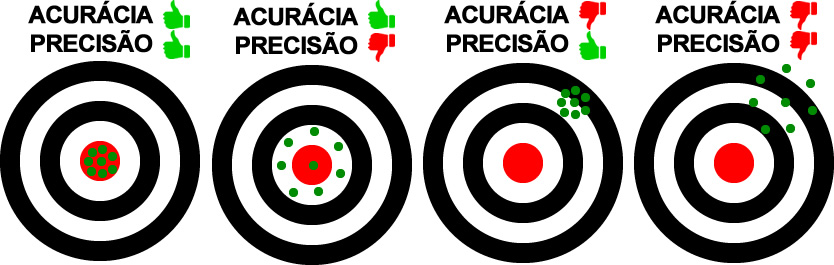
\includegraphics[width=0.9\textwidth]{modelo-monografia-rej-2018/img/PrecisaoAcuracia.jpg}
    \caption{Diferença entre Acurácia e Precisão}
    \label{fig:PrecAcur}
\end{figure}

\section{Aprendizagem Baseada em jogos - \textit{Games-based Learning}}
\label{sec:GBL}

Aprendizagem Baseada em jogos, ou GBL (pela sigla em inglês de \textit{Games-based Learning}), foi definida por alguns autores. Segundo \citeonline{tang2009introduction}, GBL faz referência a uma abordagem de aprendizagem inovadora derivada do uso de jogos de computador que tem valor educacional ou diferentes tipos de aplicação de software que usam jogos computacionais para ensino e educação. GBL's têm como finalidade o apoio à aprendizagem, a avaliação e análise de alunos e melhoria do ensino. Segundo \citeonline{monsalve2014aprendizagem}, aprendizagem baseada em jogos surge como uma alternativa de ensino que se adapta às características da pedagogia moderna na qual o estudante é um ator ativo.

Para \citeonline{monsalve2011teaching}, com a aprendizagem baseada em jogos, se pretende equilibrar entretenimento e difusão do conhecimento, motivando os estudantes a aprender enquanto jogam. \citeonline{Souza:2017:GLB:3103028.3103054} definiram \textit{GBL} como o ato de aplicar jogos com o propósito de aprender habilidades e conceitos específicos, geralmente nomeado como “jogos sérios” (jogos com fins), entretenimento educativo\footnote{Do termo, em inglês, “\textit{Edutainment}”, que seria a união de educação (\textit{Education}) e entretenimento (\textit{entertainment})} ou jogos educativos. Já \citeonline{von2009game} definiram GBL como uma abordagem lida com aplicativos de jogos que definiram resultados de aprendizagem.

Algumas plataformas de GBL foram utilizadas por autores no processo de ensino-aprendizagem. Um destes foi o de \citeonline{lot2016game}, onde abordaram o uso de GBL como avaliação formativa, com a plataforma \textbf{Zoondle}. Outras plataformas de GBL usadas foram a \textbf{EducaCross}, no trabalho de \citeonline{reis2016experiencia}, a \textbf{Timemesh}, no trabalho de \citeonline{baptista2013timemesh} e, provavelmente o mais popular, \textbf{Kahoot!}, que será usado neste projeto de pesquisa {\color{red}[Por quê escolher o Kahoot? Referenciar.]}.

\subsection{Kahoot!} \label{sec:Kahoot!}
Kahoot! é uma plataforma de aprendizado baseada em jogos usada como tecnologia educacional em escolas, universidades e outras instituições de ensino. Kahoot! foi fundada por Johan Brand, Jamie Brooker e MortenVersvik em um projeto conjunto com a Universidade Norueguesa de tecnologia e ciência \cite{kahoot2018}. Seus jogos de aprendizado, ``Kahoots'', são \textit{quizzes}, perguntas de múltipla escolha, que permitem a criação de usuários e podem ser acessados por meio de um navegador da Web, telefone ou pelo aplicativo.

Kahoot! foi projetado para a aprendizagem social, com os alunos reunidos em torno de uma tela comum, como um quadro interativo, projetor ou um monitor de computador. O site também pode ser usado por meio de ferramentas de compartilhamento de tela, como Skype ou Google hangouts. Kahoot! pode ser usado para revisar o conhecimento dos alunos, para avaliação formativa \cite{kahootFormative}, ou como uma pausa com as atividades tradicionais em sala de aula. 

A jogabilidade é simples; todos os jogadores se conectam usando um PIN de jogo gerado na tela comum e usam um dispositivo para responder a perguntas criadas pelo professor. As questões podem ter pontuações atribuídas em relação ao acerto e ao tempo para resposta. Os pontos aparecem no placar depois de cada pergunta.

Alguns trabalhos relataram os resultados encontrados ao utilizar o Kahoot! no processo de ensino. Um destes foi realizado por \citeonline{diniz2018kahoot}, que usou a ferramenta com alguns alunos de Ciência da Computação, obtendo resultados satisfatórios quanto a aceitação da ferramenta no contexto educacional.

\begin{comment}
%Artigos complementares
{\color{red}LER}
    
    \cite{chaiyo2017effect}\\
    \cite{tobias2014game}\\
    \cite{wang2015wear}\\
    \cite{connolly2012systematic}\\
    \cite{backlund2013educational}
\end{comment}
 
 No trabalho de \citeonline{petri2016quiz}, o Kahoot! foi utilizado como um \textit{quiz} com perguntas sobre Gerenciamento de Projetos, disponibilizado para alunos dos cursos de Sistemas de
Informação e Ciência da Computação como forma de revisão de conteúdo. Os autores identificaram \textit{feedbacks} positivos nos resultados encontrados. Afirmaram também que o jogo educacional cumpriu com o seu objetivo de aprendizagem por proporcionar a revisão de conhecimentos de forma divertida e motivadora.

Para os autores \citeonline{abidin2017students}, a utilização do Kahoot! foi uma estratégia de motivação para os alunos de uma faculdade de Engenharia Elétrica ao cursarem uma disciplina de programação de computadores. O conteúdo apresentado no \textit{game} era relacionado a disciplina em questão e o objetivo era possibilitar aos alunos uma experiência atrativa para a aprendizagem, pois muitos deles perdiam o entusiamo ao estudarem programação de computadores. O resultado mostrou que a grande maioria dos alunos conseguiu melhorar sua  compreensão sobre a disciplina e também se mostraram mais engajados e motivados ao final do experimento.

Outro trabalho similar foi o realizado por \citeonline{correia2017game}, que apresenta as opiniões de alunos de um programa de formação de professores (licenciatura e mestrado) sobre as vantagens e desvantagens da utilização do Kahoot! em sala de aula. Como vantagens percebidas estão a correção automática das questões e o \textit{feedback} em tempo real para os alunos e professores. Como desvantagens, foram identificados os seguintes fatores: numero limitado de caracteres tanto para o enunciado das questões quanto para as opções de respostas, além do tempo limitado de resposta.

 Considerando que alguns fatores sociais e geográficos podem afetar a aplicação e a eficiência do uso desta ferramenta, faz-se necessário avaliá-la no contexto dos estudantes brasileiros. Segundo \citeonline{pintor2014kahoot}, Kahoot! mantém as mesmas utilidades que outros métodos de resposta rápida; especialmente os \textit{clickers}, mas sem todos os problemas técnicos e logísticos destes.

\begin{comment}
\section{Introdução}
\indent\indent Este capítulo apresenta as principais características para construção de uma monografia. O referencial teórico do tema é apresentado nesta seção, ou seja, todo o conceito do trabalho deve ser descrito indicando por meio de referências, as bibliografias dos trabalhos que foram publicados sobre o tema, e que permitem o autor conceituar o assunto.
\section{Formatação da monografia}
\indent Os textos devem ser apresentados em papel branco, formato A4. Deverá ser digitado em tinta cor preta, com exceção de ilustrações. As folhas deverão apresentar margem esquerda e superior de 3 cm; direita e inferior de 2 cm. De forma geral este modelo (template) apresenta todas formatações necessárias. 
A tabela \ref{tab1} é um exemplo. 


\begin{table}[htp]
\caption{Modelo de Tabela com referência \cite{hancock1995virtual}}  
 \begin{center}
  \begin{tabular}{c|c|c|c}
   \hline
   Características & C1 & C2 & C3 \\
   \hline
   1000 & 2000 & 3000 & 1000 \\
   4000 & 2000 & 3000 & 1000 \\
   5000 & 3000 & 1000 & 1000 \\
   \hline
  \end{tabular}
  \label{tab1}
 \end{center}
\end{table}

 
\indent Tabela \ref{tab1} mostra .....

\begin{figure}[htp]
\centering
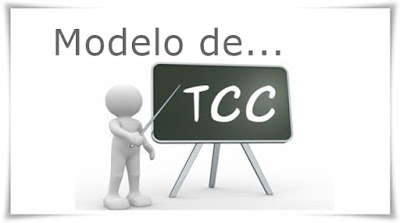
\includegraphics[scale=0.9]{img/ModeloImagem.jpg}
\caption{Modelo de Imagem \cite{pimentel1995}}
\label{modeloimg}
\end{figure}
 
	A Figura \ref{modeloimg} mostra um exemplo de como inserir uma imagem/figura e como fazer referência bibliográfica a mesma. 


Segundo \citeonline{marcoswagner_tese}, um exemplo de itens pode ser visto abaixo:

	\begin{itemize}
		\item Quanto as características da lesão:
		
	\begin{itemize}
		\item Tempo em que ocorreu a lesão:
		\item Extensão da lesão.
		\item Local da lesão.
	\end{itemize}
		\item Biografia do paciente:
		\item Idade.
		\item Diagnóstico. 
		\item Início e duração da terapia.
		\item Frequência e intensidade da terapia.
		\item Estado emocional.
		\begin{itemize}
			\item Motivação.
			\item Depressão.
		\end{itemize}
		\item Ambiente terapêutico.
		\item Comunicação.
		\item Condições físicas.
		\item Cognição; e
		\item Programa terapêutico.
	\end{itemize}




\section{Considerações Finais}
Tanto a seção Introdução como a seção Considerações Finais são opcionais na construção de um texto monográfico. Porém deve-se optar por um padrão. Coloca-se em todos os capítulos ou em nenhum...


\end{comment}
